\capitulo{3}{Conceptos teóricos}
\setsecnumdepth{subsubsection}

\section{Metabolismo de fármacos}
El metabolismo de los fármacos es el proceso mediante el cual el organismo modifica la estructura química de los medicamentos con el objetivo de facilitar su eliminación y evitar la acumulación de sustancias potencialmente tóxicas.

El principal órgano responsable de este proceso es el hígado y puede llevarse a cabo mediante diferentes mecanismos, entre ellos oxidación, reducción, hidrólisis, conjugación e isomerización. \cite{msd_metabolismo}

Una vez administrado, un fármaco puede unirse a su diana terapéutica para ejercer su acción farmacológica o ser transformado por enzimas metabolizadoras que modifican su estructura química, dando lugar a metabolitos. 

Como resultado del metabolismo pueden generarse distintos tipos de metabolitos:
\begin{itemize}
    \item \textbf{Profármacos} se introducen al organismo de forma inactiva y cuando se convierten en metabolitos acabarán como el fármaco activo con el que poder realizar el efecto deseado.
    \item \textbf{Metabolitos activos} estos seguirán con actividad biológica y pueden prolongar el efecto del medicamento original o causar efectos secundarios.
    \item \textbf{Metabolitos inactivos} que perderán su actividad biológica y tan solo se excretarán.
\end{itemize}

El proceso de metabolismo de los fármacos, en la mayoría de los casos, comprende dos fases \cite{sefh_medicamentos}, \cite{msd_metabolismo}: 
\begin{itemize}
    \item En las reacciones de fase I se altera la estructura del fármaco formando, modificando o eliminando un grupo funcional. En esta fase normalmente se utilizan enzimas provenientes del sistema enzimático del citocromo 450 (CYP450). Como resultado el fármaco se inactiva o da lugar a un metabolito activo o en el caso de los profármacos se activa, como se ha comentado previamente.
    \item En las reacciones de fase II se produce la conjugación del fármaco o de sus metabolitos con moléculas endógenas, incrementando generalmente su solubilidad en agua y facilitando su eliminación.
\end{itemize}

Hay algunos factores que alteran el metabolismo de los fármacos como por ejemplo: \cite{sefh_medicamentos}
\begin{itemize}
    \item \textbf{Factores genéticos}. Hay variaciones en los genes de cada individuo que pueden alterar a la capacidad de eliminar o procesar sustancias en el organismo.
    \item \textbf{Interacciones con otros medicamentos}. Algunos fármacos pueden inducir (acelerar) o inhibir (bloquear) las enzimas pertenecientes a CYP450, alterando el efecto de otros medicamentos administrados al mismo tiempo.
    \item \textbf{Factores dietéticos y hábitos de vida}. Cambios en ambos factores pueden alterar el metabolismo fomentandolo o, por el contrario, retrásandolo.
    \item \textbf{Enfermedades preexistentes}. Las enfermedades hepáticas, como las hepatitis o la cirrosis, pueden disminuir la capacidad metabólica del organismo. En principio, se ven más afectadas las reacciones de fase 1.
\end{itemize}


\section{Interacciones farmacológicas (fármaco-fármaco)}
Las interacciones farmácologicas de tipo fármaco-fármaco son las posibles alteraciones que pueden surgir en los efectos que deberían producir los fármacos suministrados en el organismo derivadas de la administración simultánea de dos o más medicamentos\cite{manual_msd_interacciones}.

Estas interacciones pueden incrementar o disminuir la eficacia terapéutica de los medicamentos, así como aumentar la probabilidad de aparición de efectos adversos dependiendo de las acciones que lleven a cabo las enzimas que los metabolizan.

Estas interacciones farmacológicas las podemos clasificar en dos grandes grupos: \cite{udelar_manual_farmacologia}
\begin{itemize}
    \item \textbf{Interacciones farmacodinámicas:} relacionadas con los efectos bioquímicos, celulares y fisiológicos de los fármacos en el organismo y sus mecanismos de acción.
    \item \textbf{Interacciones farmacocinéticas:} asociadas a seguir los procesos de liberación, absorción, distribución, biotransformación y eliminación de los fármacos. 
\end{itemize}


\section{Sistema enzimático del citocromo P450}
El sistema enzimático del citocromo P450 (CYP450) constituye una superfamilia de hemoproteínas con actividad oxidasa que desempeñan un papel crítico en la fase I del metabolismo xenobiótico y endógeno \cite{lorenzo2008manual}. Este sistema es el principal responsable de la depuración metabólica de fármacos, la activación de profármacos y la generación de interacciones farmacológicas adversas.

Las enzimas CYP se localizan predominantemente en la membrana del retículo endoplásmico liso de los hepatocitos, aunque también presentan una expresión significativa en el tejido intestinal, los pulmones o los riñones. Su función principal es catalizar reacciones de oxidación pertenecientes a la fase I del metabolismo de los fármacos, facilitando posteriormente su eliminación o su transformación mediante las reacciones de fase II \cite{sefh_medicamentos}, \cite{msd_metabolismo}.

\subsection{Importancia clínica y enzimas principales}
El sistema CYP450 desempeña un papel fundamental en farmacología debido a que determina la velocidad con la que los medicamentos son metabolizados y eliminados del organismo. La actividad de estas enzimas puede variar entre individuos debido a factores genéticos, fisiológicos o ambientales, lo que provoca diferencias en la respuesta a un mismo tratamiento farmacológico.

Además, muchas interacciones farmacológicas están relacionadas con la capacidad de determinados medicamentos para inhibir o inducir la actividad de las enzimas CYP450. Estas alteraciones pueden modificar las concentraciones plasmáticas de otros fármacos administrados simultáneamente, aumentando el riesgo de efectos adversos o reduciendo la eficacia terapéutica.

Aunque se han identificado decenas de isoenzimas humanas, un grupo selecto de seis isoformas pertenecientes a las familias CYP1, CYP2 y CYP3 es responsable del metabolismo de la mayor parte de los fármacos utilizados en la práctica clínica actual, esto se puede observar en el gráfico \ref{fig:grafica_cyp}. Estas son las siguientes \cite{zanger2013cytochrome}:

\paragraph{CYP3A4}
Es la enzima metabólica más importante de toda la superfamilia, constituyendo la enzima por la que mas se metabolizan los fármacos comercializados. Se encuentra principalmente en el hígado y en el intestino.

\paragraph{CYP2D6}
Participa en el metabolismo de aproximadamente el 20 porciento de los fármacos comercializados afectando a familias críticas como los antidepresivos, antipsicóticos y analgésicos opioides. Destaca por presentar una elevada variabilidad genética entre individuos, lo que puede originar metabolizadores lentos, normales o ultrarrápidos. 

\paragraph{CYP2C9}
Interviene en el metabolismo de medicamentos de uso frecuente como los anticoagulantes y algunos antiinflamatorios no esteroideos. Las variaciones genéticas en esta enzima pueden afectar significativamente a la dosis necesaria de algunos tratamientos.

\paragraph{CYP2C19}
Pertenece a la familia CYP2 como el CYPD6 y el CYP2C9. Metaboliza fármacos como el clopidogrel, el omeprazol o determinados antidepresivos, se trata de la enzima por la que son metabolizados menos fármacos de todas las elegidas. Al igual que CYP2D6, presenta polimorfismos genéticos que pueden alterar la respuesta terapéutica.

\paragraph{CYP1A2}
Esta enzima pertenece al grupo de las CYP1. Su actividad puede verse modificada por factores ambientales como el tabaquismo.

\paragraph{CYP3A5} 
Es una enzima perteneciente a la subfamilia CYP3A. Junto con CYP3A4, es una de las principales enzimas responsables del metabolismo de medicamentos en humanos. La mayoría de personas no expresan el CYP3A5 debido a la gran cantidad de polimorfismos que posee, por lo tanto no es considerada tan relevante como el CYP3A4 \cite{lamba2012pharmgkb}. Sin embargo, para las personas que la expresan esta encima el CYP3A5 puede representar más de la mitad de toda la actividad CYP3A hepática, influyendo significativamente en la velocidad de eliminación de determinados medicamentos. \cite{wang2001abundance}

\begin{figure}[htbp!]
    \centering
    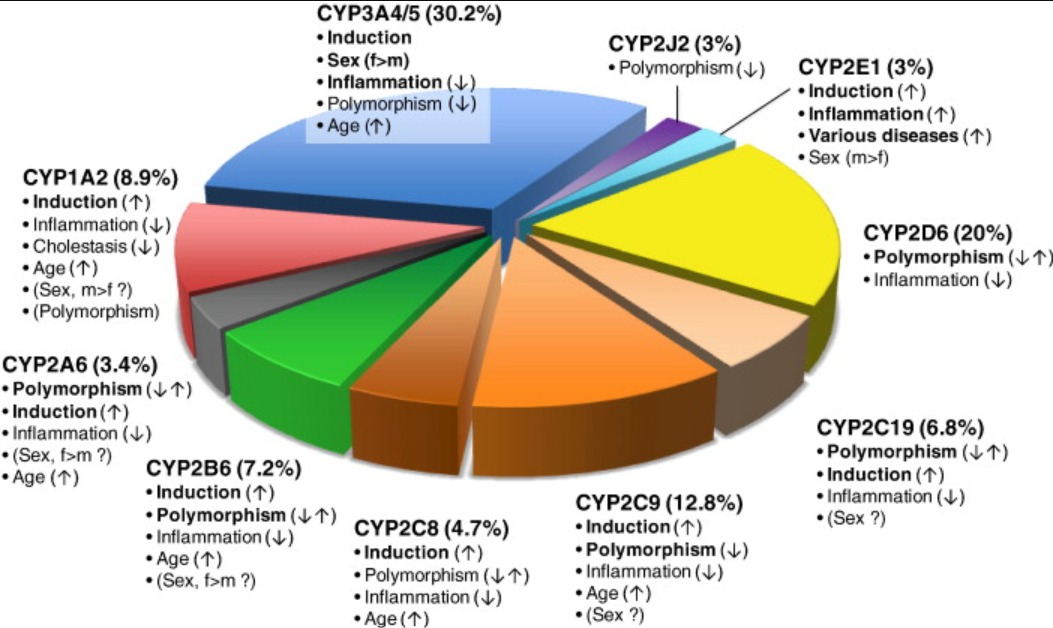
\includegraphics[width=0.7\textwidth]{img/grafica_cyp.jpeg} 
    \caption{Regulación de la expresión génica y actividades enzimáticas del CYP (fuente: \cite{zanger2013cytochrome}).}
    \label{fig:grafica_cyp}
\end{figure}

\subsection{Inducción e inhibición enzimática}
Las enzimas del sistema CYP450 pueden verse afectadas por la presencia de determinados fármacos o sustancias externas.

La inducción enzimática consiste en un aumento de la actividad metabólica de una enzima, lo que provoca una eliminación más rápida de los medicamentos metabolizados por dicha vía y, en consecuencia, una posible disminución de su efecto terapéutico.

Por el contrario, la inhibición enzimática reduce la actividad de la enzima, aumentando las concentraciones plasmáticas del fármaco afectado y el riesgo de aparición de efectos adversos o toxicidad.

Estos fenómenos constituyen uno de los principales mecanismos responsables de las interacciones farmacológicas de tipo farmacocinético.

Debido a que numerosos medicamentos comparten las mismas vías metabólicas, el sistema CYP450 constituye uno de los principales responsables de las interacciones fármaco-fármaco. Cuando dos o más fármacos son administrados simultáneamente, pueden competir por una misma enzima, inducir su actividad o inhibirla, alterando las concentraciones plasmáticas de alguno de ellos.


\section{Sistema de Clasificación Anatómica, Terapéutica y Química (ATC)}
El Sistema ATC es un estándar internacional de codificación de sustancias farmacéuticas y medicamentos \cite{whocc_home}. Instaurado y mantenido por el Centro Colaborador de la Organización Mundial de la Salud (OMS) para la Metodología de Estadísticas sobre medicamentos.
Este sistema constituye una herramienta fundamental en la informática biomédica para la interoperabilidad de datos clínicos, la farmacovigilancia y el análisis epidemiológico \cite{who_atc_classification}.

El objetivo principal del sistema ATC es servir como un instrumento estandarizado para la presentación de estadísticas sobre el consumo de medicamentos a nivel global, permitiendo la comparación armonizada de datos entre diferentes regiones, centros hospitalarios y periodos de tiempo \cite{who_atc_methodology}.

A cada fármaco le corresponde un único código ATC que lo clasifica según su principal indicación terapéutica. Los principio activos contenidos en los fármacos pueden tener más de un código ATC, en el caso en el que éste se emplee en indicaciones o en formas farmacéuticas diferentes, sin embargo, no hay un mismo código ATC completo asociado a mas de un principio activo\cite{sacyl_uso_racional}

\subsection{Estructura y Jerarquía del Código ATC}
El sistema ATC se organiza de forma jerárquica en cinco niveles independientes. Cada principio activo recibe un código alfanumérico único de 7 caracteres que detalla desde el sistema orgánico sobre el que actúa hasta su estructura química específica \cite{whocc_structure} .

La arquitectura de dichos niveles se estructura de la siguiente manera  \cite{whocc_structure} \cite{who_atc_classification} :
\begin{enumerate}
    \item \textbf{Nivel Anatómico.} Consta de una letra que indica el grupo anatómico principal, es decir, el órgano o sistema sobre el que actúa el fármaco (en total existen 14 grupos principales).
    \item \textbf{Nivel Terapéutico} Formado por un código numérico de dos dígitos que identifica el grupo terapéutico principal.
    \item \textbf{Nivel Farmacológico/Terapéutico.} Constituido por una letra que especifica el subgrupo terapéutico o farmacológico.
    \item \textbf{Nivel Químico.} Compuesto por una letra que define el subgrupo químico, terapéutico o farmacológico detallado.
    \item \textbf{Nivel Sustancia Química.} Formado por un código numérico de dos dígitos que designa de manera exclusiva la sustancia química o principio activo individual.
\end{enumerate}


\section{Herramientas para la Base de Datos y la visualización}
Para la generación de los conjuntos de datos consolidados \texttt{DDI\_sea.csv} y \texttt{efectos\_adversos.csv}, se ha extraído e integrado la información procedente de las plataformas de referencia internacional DrugBank \cite{drugbank}, SIDER \cite{sider} y el portal oficial CIMA \cite{cima}. 

Por otro lado, la visualización de los resultados y el análisis de las interacciones farmacológicas se ha implementado mediante el entorno de desarrollo Dash \cite{dash_framework}. Este enfoque permite desplegar un cuadro de mando interactivo que facilita la interpretación de las interacciones y sus causas etiológicas por parte del personal facultativo de manera intuitiva.

A continuación, se detallan las características y el propósito analítico de cada una de las herramientas seleccionadas

\subsection*{DrugBank}
DrugBank es una base de datos biológica y bioinformática de acceso público y gratuito para fines académicos que centraliza información sumamente detallada sobre medicamentos y sus dianas terapéuticas.
En este proyecto, se ha utilizado para recuperar los nombres de los principios activos y sus correspondientes códigos ATC. Asimismo, permite identificar las enzimas metabólicas asociadas, las dianas biológicas hacia las que se dirigen los compuestos y sus respectivos mecanismos de acción.

\subsection*{CIMA}
CIMA son las siglas del Centro de Información Online de Medicamentos de la Agencia Española de Medicamentos y Productos Sanitarios (AEMPS). Es una base de datos pública, oficial y gratuita que contiene todos los medicamentos autorizados en España, así como aquellos cuya autorización ha sido revocada, suspendida o caducada.
En el marco de este trabajo, se han aplicado técnicas de extracción automatizada de datos (web scraping) sobre sus fichas técnicas oficiales. El objetivo principal de este proceso es resolver ambigüedades en aquellos principios activos para los que DrugBank identifica múltiples vías metabólicas, logrando así determinar con precisión cuál es la enzima principal responsable de su metabolismo.

\subsection*{SIDER}
SIDER es una base de datos bioinformática de acceso público cuyo propósito principal es centralizar, registrar y conectar información estructurada sobre los efectos secundarios de los medicamentos y sus frecuencias de aparición clínicamente documentadas por mas de una fuente. Sirve como un recurso complementario a plataformas como DrugBank.
Esta plataforma se ha empleado de forma complementaria para asociar a cada principio activo su perfil de efectos secundarios y la probabilidad de manifestación de los mismos. Ademas, integra la codificación estandarizada ATC para cada sustancia, lo que facilita la recuperación de su información.

\subsection*{DASH}
El entorno de desarrollo de DASH tiene la capacidad de transformar almacenes de datos biomédicos complejos en interfaces analíticas comprensibles para la visualización de los resultados. Se ha consolidado como un framework de código abierto fundamental para la construcción de aplicaciones web analíticas e interactivas utilizando exclusivamente lenguajes de programación científicos como Python, R o Julia.


\section{Estado del arte y trabajos relacionados.}
En los últimos años se han desarrollado numerosas herramientas destinadas a detectar posibles interacciones entre medicamentos (Drug-Drug Interactions, DDI), tanto en el ámbito investigador como en aplicaciones de uso clínico. La mayoría de estas soluciones permiten consultar la posible interacción entre dos o más principios activos, proporcionando un nivel de gravedad junto con recomendaciones clínicas. Sin embargo, pocas ofrecen una explicación detallada del mecanismo farmacocinético responsable de la interacción o permiten explorar alternativas terapéuticas de forma integrada.

Uno de los trabajos académicos mas relevantes es el publicado en 2024 en PubMed \cite{pubmed_39180399}, donde se presenta un sistema basado en información farmacológica para el estudio de interacciones entre fármacos. El trabajo pone de manifiesto la importancia de integrar bases de datos biomédicas y mecanismos moleculares para mejorar la interpretación de las interacciones de medicamentos. 

En el ámbito de las bases de datos especializadas destaca DDInter2 \cite{ddinter_database}, una plataforma que recopila información procedente de diferentes fuentes bibliográficas y bases de datos farmacológicas. Esta herramienta ofrece una gran cobertura de interacciones conocidas, indicando el mecanismo implicado, el nivel de evidencia y referencias bibliográficas. Su principal fortaleza reside en la amplitud de la información disponible, aunque la cantidad de datos mostrados puede dificultar la interpretación rápida por parte de usuarios no especializados.

Entre las herramientas de uso clínico más extendidas se encuentran los comprobadores de interacciones de Medscape \cite{medscape_checker}, RxList \cite{rxlist_checker} y Drugs.com \cite{drugs_checker}. Estas plataformas permiten consultar rápidamente posibles interacciones entre medicamentos y clasificarlas según su gravedad clínica. Además, suelen incorporar recomendaciones generales para el profesional sanitario. Sin embargo, su funcionamiento se basa principalmente en mostrar el resultado de la interacción y una descripción textual, sin explicar de manera detallada el razonamiento seguido para alcanzar dicha clasificación.

La herramienta desarrollada en este Trabajo Fin de Grado adopta un enfoque diferente al de las soluciones existentes. En lugar de limitarse a indicar si existe o no una interacción, analiza el metabolismo de ambos principios activos utilizando la información contenida en DrugBank sobre enzimas metabolizadoras, prestando especial atención a las enzimas CYP más relevantes (CYP3A4, CYP3A5, CYP2D6, CYP2C9, CYP2C19 y CYP1A2). A partir de esta información determina un nivel de riesgo (bajo, medio o alto) en función de la coincidencia de las enzimas implicadas y de si estas han sido identificadas como principales en el metabolismo de cada fármaco.

Además de clasificar el riesgo, proporciona una explicación del motivo de la interacción, indicando las enzimas compartidas y el papel que desempeña cada principio activo sobre ellas (sustrato, inhibidor o inductor). Esta característica aporta un componente de interpretabilidad que no suele encontrarse en los comprobadores comerciales, permitiendo comprender el mecanismo farmacocinético responsable de la posible interacción.

Otra contribución diferencial consiste en la incorporación de un módulo de búsqueda de alternativas terapéuticas basado en la clasificación ATC. Cuando se detecta una interacción de riesgo medio o alto, el sistema identifica principios activos pertenecientes al mismo grupo terapéutico y evalúa automáticamente todas las combinaciones posibles hasta encontrar aquellas cuya interacción se clasifica como de bajo riesgo. De esta forma, la herramienta no solo identifica el problema, sino que propone posibles soluciones consideradas seguras para el algoritmo.

Finalmente, la aplicación integra información sobre efectos adversos procedente de la base de datos SIDER, mostrando gráficamente los efectos secundarios más frecuentes asociados a los códigos ATC de referencia. Esta funcionalidad proporciona información adicional que puede resultar útil durante la valoración de posibles alternativas terapéuticas.
